\documentclass{beamer}
\usepackage{booktabs}
\usepackage{pdfpages}
\usepackage{mathtools}
\usepackage{enumerate}
\usepackage{multirow,tabularx}
\usepackage{booktabs}
\usepackage{pdfpages}
\usepackage{proof}
\usepackage{cancel}
\usepackage{chronology}
\usepackage{graphicx}
\usepackage{ulem}
\usepackage{amsmath}
\usepackage{amssymb}
\usepackage{color}
\usepackage{animate}
\usepackage{xr}

\PassOptionsToPackage{usenames,dvipsnames,svgnames}{xcolor}  
\usepackage{tikz}
\usepackage{tkz-graph}


\usepackage{wasysym}
\usepackage{proof}
\usepackage{cancel}
\usepackage{chronology}
\usepackage{graphicx}
\usepackage{ulem}
\usepackage{amsmath}
\usepackage{amssymb}
\usepackage{color}
\usepackage{xcolor}
\usepackage{soul}
%\usepackage{pstricks}
\setbeamertemplate{navigation symbols}{}

\newcommand{\norm}[1]{\left\lVert#1\right\rVert}
\newcommand{\el}{$\mathcal{EL}^{++}$}
\renewcommand{\Re}{\mathbb{R}}
\newcommand{\BigO}[1]{\ensuremath{\operatorname{O}\bigl(#1\bigr)}}
\newcommand{\myul}[2][blue]{\sethlcolor{#1}\hl{#2}\setulcolor{black}}

\newcommand<>{\cunderline}[3]{\only<#1>{#3}\only<#2>{\underline{#3}}}
\newcommand<>{\cem}[3]{\only<#1>{#3}\only<#2>{\ul{#3}}}
\newcommand<>{\cgray}[3]{\only<#1>{#3}\only<#2>{\textcolor{gray}{#3}}}
\newcommand<>{\colorize}[4]{\only<#1>{#4}\only<#2>{\textcolor{#3}{#4}}}

\setbeamertemplate{navigation symbols}{\insertslidenavigationsymbol}
%\setbeamertemplate{navigation symbols}{}
% \addtobeamertemplate{navigation symbols}{}{%
%     \usebeamerfont{footline}%
%     \usebeamercolor[fg]{footline}%
%     \hspace{1em}%
%     \insertframenumber/\inserttotalframenumber
% }

\mode<presentation>
{
\usecolortheme{crane}
%\useoutertheme{split}

\expandafter\def\expandafter\insertshorttitle\expandafter{%
  \insertshorttitle\hfill%
  \insertframenumber\,/\,\inserttotalframenumber}

\usefonttheme[onlysmall]{structurebold}
}
\renewcommand{\em}{\itshape}
\usepackage{pifont}
\definecolor{purple}{rgb}{1,0,1}
\definecolor{dred}{rgb}{0.7,0,0}
\definecolor{myred}{rgb}{1,0,0}
\definecolor{dblue}{rgb}{0,0,0.7}
\definecolor{dgreen}{rgb}{0,0.5,0}
\definecolor{myyellow}{rgb}{1,1,0}
\newcommand{\parents}[1]{parents(#1)}
\setbeamertemplate{itemize item}[ball]


% \mode<presentation>
% {
% \useinnertheme[shadow=true]{rounded}
% \useoutertheme{infolines}
% \usecolortheme{dove}
% \setbeamerfont{block title}{size={}}
% }

\title[Relational]{Relational and semantic data}

%\author{Robert Hoehndorf and Maxat Kulmanov}


\date{}

\begin{document}

\begin{frame}
  \titlepage
\end{frame}

\section{Introduction}

\begin{frame}
  \frametitle{(Background) knowledge, machine learning, and AI}
  \begin{itemize}
  \item knowledge bases containing background knowledge are everywhere
  \item rich formal characterization (axioms)
  \item how can they be used for (predictive) data analysis?
    \begin{itemize}
    \item ``fuzzy'', similarity-based search
    \item predictive analysis and machine learning
    \end{itemize}
  \end{itemize}
\end{frame}

\begin{frame}
  \frametitle{Learning goals}
  \begin{itemize}
  \item machine learning with structured background knowledge
  \item unsupervised or supervised:
    \begin{itemize}
    \item here: mostly unsupervised {\em feature} learning
    \item ``deep'' learning
    \end{itemize}
  \item focus on existing tools and methods
    \begin{itemize}
    \item Jupyter Notebooks and code examples
    \item mOWL library
    \end{itemize}
  \item not covered:
    \begin{itemize}
    \item extracting knowledge (axioms, definitions) from data
    \item (most) natural language processing
    \item reasoning and deduction
    \item machine learning theory
    \end{itemize}
  \end{itemize}
\end{frame}

\begin{frame}
  \frametitle{Agenda}
  \begin{itemize}
  \item Introduction: knowledge bases and graphs
  \item Semantic similarity
  \item Machine learning with background knowledge
  \item applications
  \item (most hands-on components based on the mOWL library)
  \end{itemize}
\end{frame}

\begin{frame}
  \frametitle{Classifying diseases}
  \begin{itemize}
  \item Francois Bossier de Lacroix (18th century): Nosologia
    Methodica
  \item William Cullen of Edinburgh (1785): Synopsis nosologiae
    methodica
  \item William Farr (1837): improved classification, standardization,
    international collaboration
  \item Jaques Bertillon (1893): International (Bertillon)
    Classification of Causes of Death
  \item 1900: International Classification of Diseases (ICD) version 1
  \item 2022: International Classification of Diseases (ICD) version 11
  \end{itemize}
\end{frame}

\begin{frame}
  \frametitle{Classifying diseases}
  Breast cancer:
  \begin{itemize}
  \item specific anatomy
  \item histopathology
  \item grade and stage
  \item molecular subtype
  \item celltype of origin
  \item (etiology)
  \end{itemize}
\end{frame}

\begin{frame}
  \frametitle{Relational data}
  \centerline{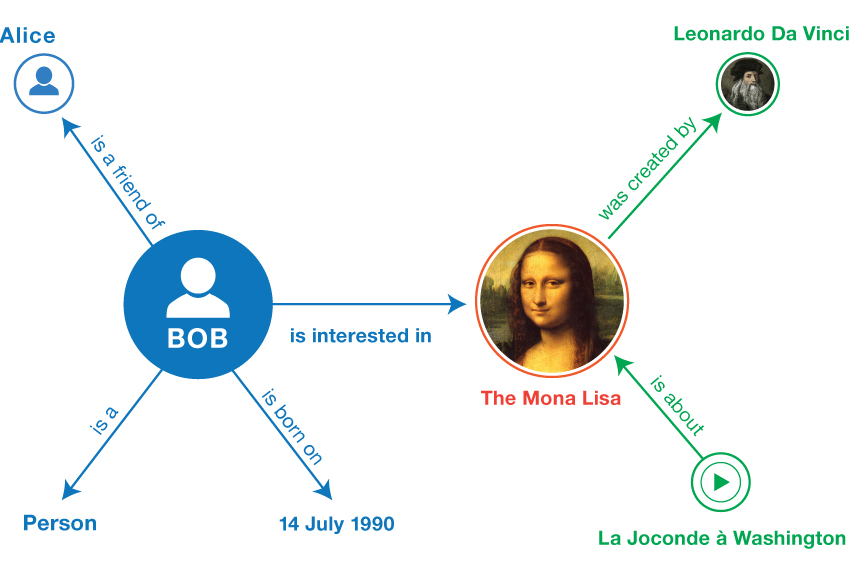
\includegraphics[height=.8\textheight]{example-graph.jpg}}
  \begin{itemize}
  \item entities
  \item relations
  \item triple: subject, predicate, object
  \end{itemize}
  But what do all these names/relations mean?
\end{frame}

\begin{frame}
  \frametitle{Relational data}
  \centerline{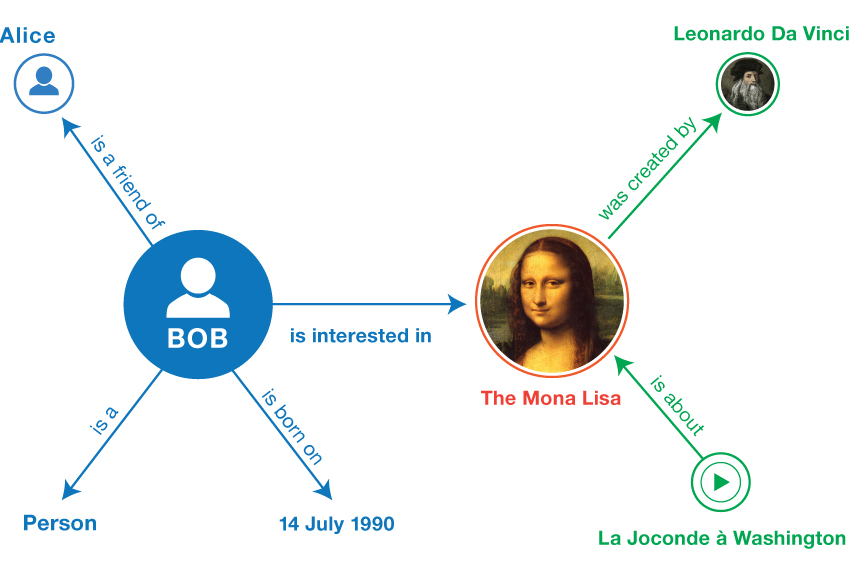
\includegraphics[height=.8\textheight]{example-graph.jpg}}
  \begin{itemize}
  \item every ``breast cancer'' is a type of cancer
  \item every person has exactly two parents
  \item how many parents does Bob have?
  \end{itemize}
\end{frame}

% \begin{frame}
%   \frametitle{Ontologies}
%   \begin{itemize}
%   \item Specific artifacts expressing the intended meaning of a
%     vocabulary in terms of primitive categories and relations
%     describing the nature and structure of a domain of discourse
%     \begin{itemize}
%     \item in order to account for the competent use of vocabulary in
%       real situations (such as annotations in databases, etc.)
%     \end{itemize}
%   \item the intended meaning of {\em primitive} categories and
%     relations is expressed through axioms (axiomatic method, Tarski)
%   \end{itemize}
% \end{frame}

\begin{frame}
  \frametitle{Axioms}
  \begin{itemize}
  \item {\em classes} represent kinds of things in the world
    \begin{itemize}
    \item {\em Arm}, {\em Apoptosis}, {\em Influenza}, {\em Homo
        sapiens}, {\em Drinking behavior}, {\em Membrane}
    \end{itemize}
  \item {\em instances} of classes are individuals satisfying the
    classes' intension
    \begin{itemize}
    \item my arm, the influenza I had last year, one ethanol molecule, etc.
    \end{itemize}
  \item {\em relations} between instances arise from interactions,
    configurations, etc., of individuals
    \begin{itemize}
    \item my arm is {\bf part of} me, the {\bf duration of} my
      influenza was 10 days
    \end{itemize}
  \item {\em axioms} specify the conditions that instances of a class
    must satisfy
    \begin{itemize}
    \item every instance of {\em Hand} is a {\bf part of} an instance
      of {\em Arm}
    \end{itemize}
  \end{itemize}
\end{frame}

\begin{frame}
  \frametitle{Ontologies}
  \centerline{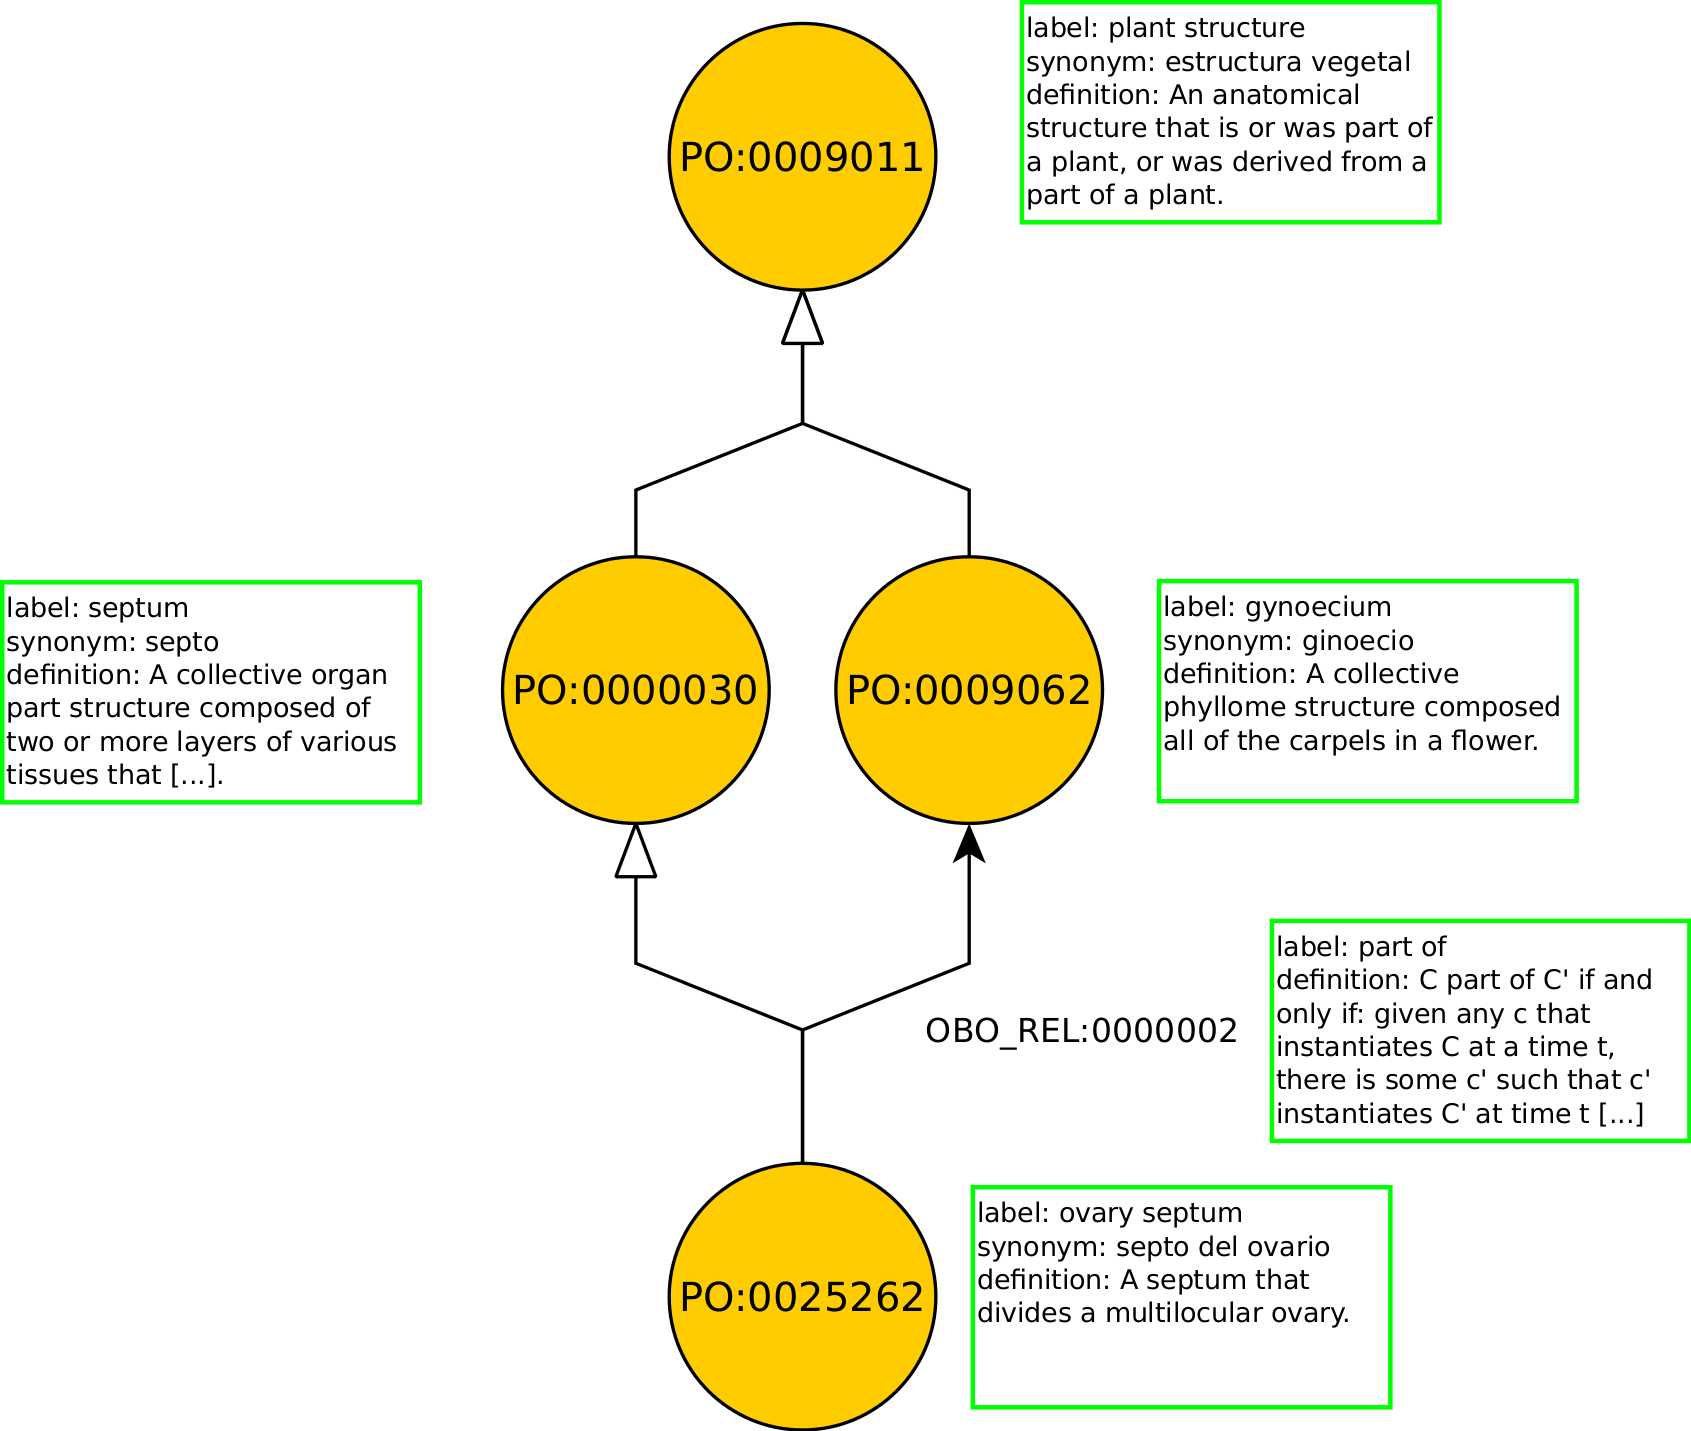
\includegraphics[height=.8\textheight]{plant-ontology-sample.png}}
\end{frame}

% \begin{frame}
%   \frametitle{Ontologies provide background knowledge}
%   \centerline{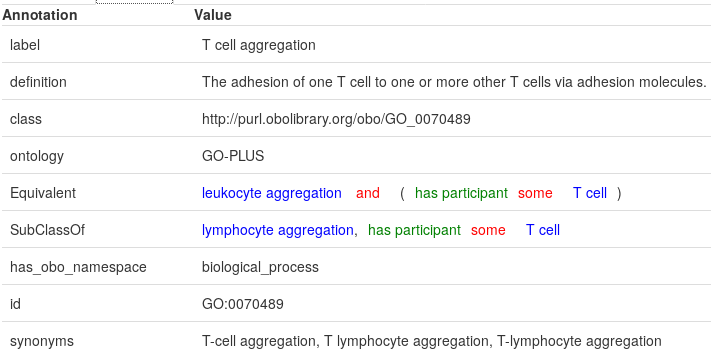
\includegraphics[width=.8\textwidth]{t-cell-aggregation.png}}
% \end{frame}

% \begin{frame}
%   \frametitle{Ontologies provide background knowledge}
%   \centerline{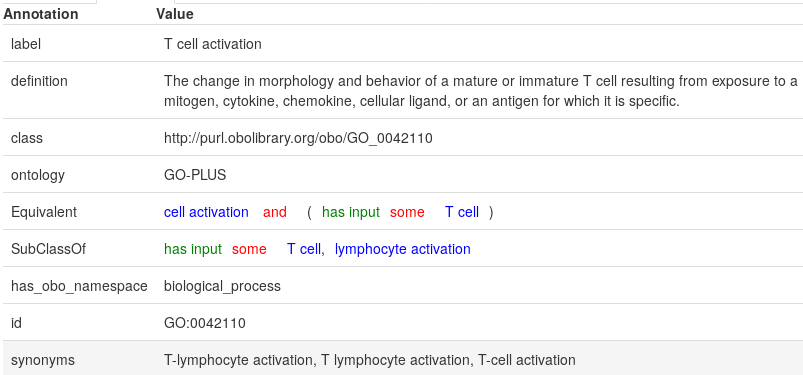
\includegraphics[width=.8\textwidth]{t-cell-activation.png}}
% \end{frame}

\begin{frame}
  \frametitle{Semantic similarity: some examples}
  \begin{itemize}
  \item Are cyclin dependent kinases {\em functionally} more similar
    to lipid kinases or to riboflavin kinases? How about {\em
      phenotypically}?
  \item Which protein in the {\em mouse} is functionally most similar
    to the zebrafish {\em gustducin} protein?
  \item Which mouse knockout resembles {\em Bardet-Biedl Syndrome 8}?
  \item Are there mouse knockouts that resemble the side effects of
    diclofenac?
  \item Which genetic disease produces similar symptoms to ebola?
  \item Does functional similarity correlate with phenotypic
    similarity?
  \end{itemize}
\end{frame}

\begin{frame}
  \frametitle{Semantic similarity}
  semantic similarity measures:
  \begin{itemize}
  \item for words, terms, classes
  \item role of background knowledge:
    \begin{itemize}
    \item statistical/distributional semantics, large corpora
    \item ontologies: (graph) topology
    \end{itemize}
  \item similarity measures: hand-crafted or data-driven?
  \end{itemize}
\end{frame}

\begin{frame}
  \frametitle{Semantic similarity or machine learning}
  \begin{itemize}
  \item semantic similarity measures are mostly hand-crafted
    \begin{itemize}
    \item capture certain intuition about what constitutes
      ``similarity''
    \item different measures for different kinds of similarity
    \item usually interpretable (and explainable)
    \end{itemize}
    \pause
  \item machine learning methods are mostly data-driven
    \begin{itemize}
    \item the architecture of the model is still hand-crafted
    \item usually hard to interpret
    \end{itemize}
  \end{itemize}
\end{frame}

\begin{frame}
  \frametitle{Knowledge bases and graphs}
  \begin{itemize}
  \item semantic similarity measures {\em and machine learning models}
    on knowledge bases (ontologies) can be graph-based, feature-based,
    or model-based
    \begin{itemize}
    \item graph-based: ontology as a graph
    \item feature-based: extract (or obtain) features for
      classes/relations
    \item model-based: define similarity within (special) $\Sigma$-algebras
    \end{itemize}
  \end{itemize}
\end{frame}

\end{document}

%%% Local Variables:
%%% mode: latex
%%% TeX-master: t
%%% End:
